\chapter{Ugeopgave 5}
\label{cha:ugeopgave-5}

\section{Del 1}
\label{sec:del-1}

Hvis \emph{hidden surface}-algoritmen ikke er aktiveret, f�s
resultatet p� figur \ref{fig:5-1-1}. N�r \emph{hidden
  surface}-algoritmen aktiveres, fjernes kassen, som det kan ses p�
figur \ref{fig:5-1-2}.

\begin{figure}[hp]
\centering
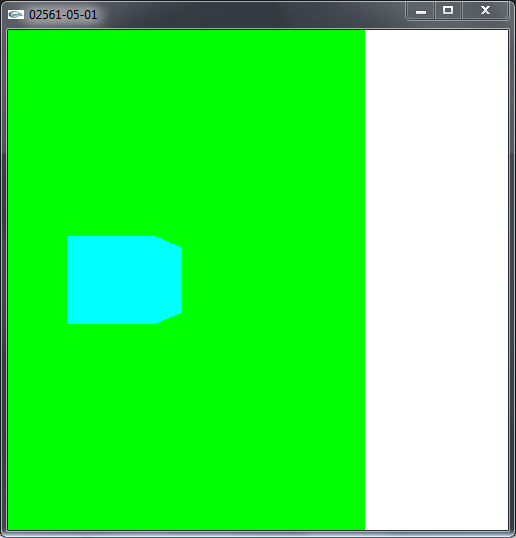
\includegraphics[width=8cm]{../exercise5/screenshots/part1_1.png}
\caption{Ingen \emph{hidden surface}}
\label{fig:5-1-1}
\end{figure}

\begin{figure}[hp]
\centering
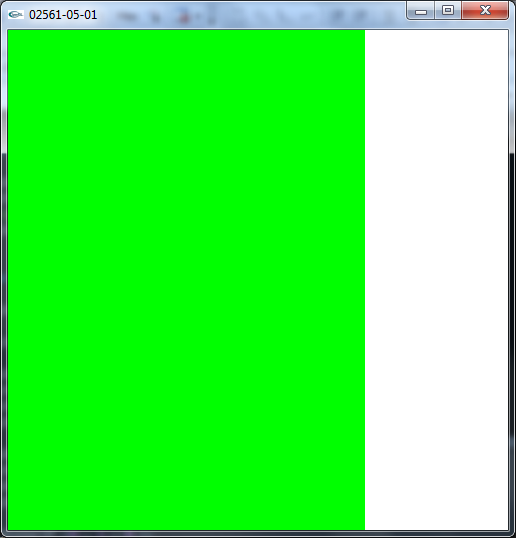
\includegraphics[width=8cm]{../exercise5/screenshots/part1_2.png}
\caption{Aktiveret \emph{hidden surface}}
\label{fig:5-1-2}
\end{figure}

\section{Del 2}
\label{sec:del-2}

P� figur \ref{fig:5-2-1} er \emph{viewing frustrum}'et �ndret, s� den
gr�nne flade er klippet v�k.

Figur \ref{fig:5-2-2} viser resultatet af at have lavet et ekstra
\emph{clipping} plan. Planet er det plan, der udsp�ndes af de to
linjer, defineret i programmet ($(0,0,0) \rightarrow (15,0,0)$ og
$(0,0,0) \rightarrow (0,15,0)$).

\begin{figure}[hp]
\centering
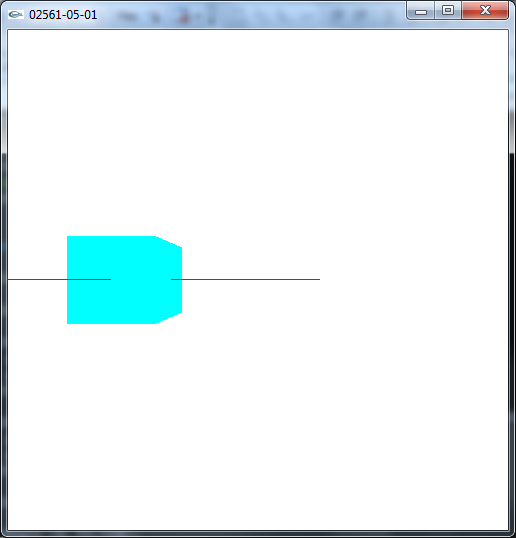
\includegraphics[width=8cm]{../exercise5/screenshots/part2_1.png}
\caption{�ndret \emph{viewing frustrum}}
\label{fig:5-2-1}
\end{figure}

\begin{figure}[hp]
\centering
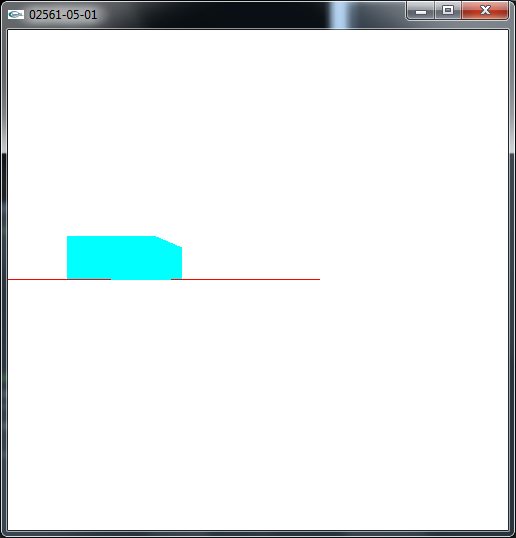
\includegraphics[width=8cm]{../exercise5/screenshots/part2_2.png}
\caption{Ekstra \emph{clipping plane}}
\label{fig:5-2-2}
\end{figure}

\section{Del 3}
\label{sec:del-3}

OpenGL muligg�r forskellige filtreringsteknikker n�r man bruger
teksturer. Den ene er \emph{point sampling}, hvor der laves et direkte
``opslag'' i teksturen p� �t punkt for at finde ud af hvilken farve
der skal renderes. Bruger man \emph{linear filtering} i stedet, vil
der blive lavet et v�gtet gennemsnit af omr�det omkring det �nskede
punkt, hvorefter gennemsnitsfarven bruges som den endelige farve. Ved
\emph{point sampling} er der st�rre chance for \emph{aliasing} end ved
\emph{linear filtering}. I begge tilf�lde vil \emph{aliasing} dog
kunne minimeres ved brug af \emph{mipmapping}. \emph{Mipmapping} er en
metode, der forbedrer billedkvaliteten ved at bruge forskellige
st�rrelser teksturer alt efter st�rrelsen p� det projicerede
omr�de. Dermed kan man undg� noget \emph{aliasing}, da man automatisk
kan smide uoverfl�dig, og \emph{alias}-genererende, information v�k.

Resultatet af at k�re programmet \texttt{02561-05-03-2009} med
\emph{linear filtering} kan ses p� figur \ref{fig:5-3-1}, mens
\emph{point sampling} demonstreres p� figur \ref{fig:5-3-2}. I
\emph{point sampling}-eksemplet er der tydelig \emph{aliasing} mens
der i \emph{linear filtering}-eksemplet vises en lettere udtv�ret
tekstur.

\begin{figure}[hp]
\centering
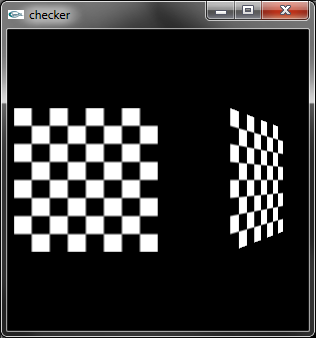
\includegraphics[width=8cm]{../exercise5/screenshots/part3_1.png}
\caption{\emph{Linear filtering}}
\label{fig:5-3-1}
\end{figure}

\begin{figure}[hp]
\centering
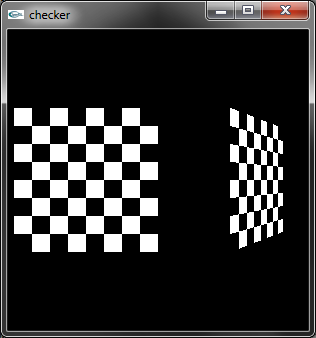
\includegraphics[width=8cm]{../exercise5/screenshots/part3_2.png}
\caption{\emph{Point sampling}}
\label{fig:5-3-2}
\end{figure}

Ved \texttt{GL\_MODULATE} bestemmes farven af et punkt ved multiplikation af
teksturens farve og den farve, punktet ville have f�et af den normale
shader.

Bruges der \texttt{GL\_DECAL} i stedet, bestemmer teksturen fuldst�ndig
punktets farve. Det samme g�r sig g�ldende ved brug af
\texttt{GL\_REPLACE} - her bruges alpha-informationer bare ogs�,
hvilket de ikke g�r ved \texttt{GL\_DECAL}.

\section{Del 4}
\label{sec:del-4}

Resultatet af at \emph{mappe} teksturen i forholdet $10:1$
(dvs. objektkoordinaterne $(10.0,~6.0)$ bliver til
teksturkoordinaterne $(1.0,~0.6)$) kan ses p� figur \ref{fig:5-4-1}.

$5:1$-mapping ($(10.0,~6.0) \rightarrow (2.0,~1.2)$) med
\emph{clamping} kan ses p� figur \ref{fig:5-4-2} mens forts�ttelse
(vha. \texttt{GL\_REPEAT}) ses p� figur \ref{fig:5-4-3}.

\begin{figure}[hp]
\centering
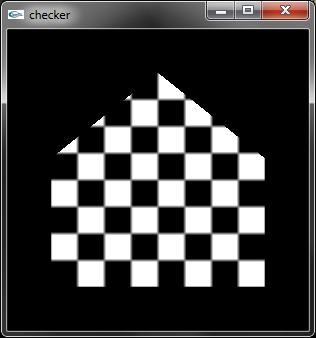
\includegraphics[width=8cm]{../exercise5/screenshots/part4_1.png}
\caption{$10:1$ mapping}
\label{fig:5-4-1}
\end{figure}

\begin{figure}[hp]
\centering
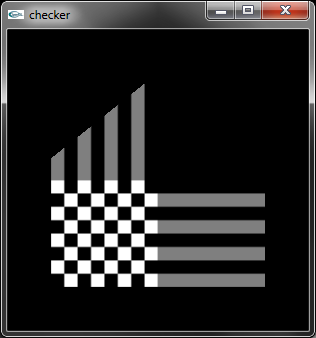
\includegraphics[width=8cm]{../exercise5/screenshots/part4_2.png}
\caption{$5:1$ mapping med \emph{clamping}}
\label{fig:5-4-2}
\end{figure}

\begin{figure}[hp]
\centering
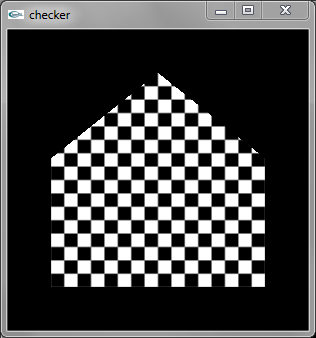
\includegraphics[width=8cm]{../exercise5/screenshots/part4_3.png}
\caption{$5:1$ mapping med forts�ttelse}
\label{fig:5-4-3}
\end{figure}

\section{Del 5}
\label{sec:del-5}

Resultatet af at rotere teksturen $45 \degree$ om z-aksen kan ses p�
figur \ref{fig:5-5-1}. Roteringen er foretaget ved brug af f�lgende
kode:

\begin{verbatim}
glMatrixMode(GL_TEXTURE);
glLoadIdentity();
glRotatef(45.0, 0.0, 0.0, 1.0);
\end{verbatim}

\begin{figure}[hp]
\centering
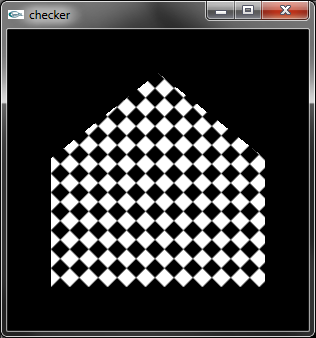
\includegraphics[width=8cm]{../exercise5/screenshots/part5.png}
\caption{Rotering af tekstur}
\label{fig:5-5-1}
\end{figure}

%%% Local Variables: 
%%% mode: latex
%%% TeX-master: "report_main"
%%% End: 